\documentclass{standalone}
\usepackage{tkz-graph, calc}
\usetikzlibrary{arrows,graphs,matrix,positioning, arrows.meta}



\begin{document}


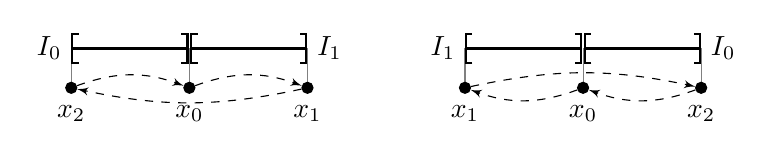
\begin{tikzpicture}

\tikzset{vertex/.style = {shape=circle, fill=black,draw,minimum size=4pt, inner sep=0pt}}
\tikzset{edge/.style = {->,> = latex'}}
\tikzset{interval/.style = {<->,> = {Bracket[length=0.8mm, width=4mm]}, line width = 0.8pt}}

%help lines
\draw[gray] (0, 0) -- (0, 0.5);
\draw[gray] (1.5, 0) -- (1.5, 0.5);
\draw[gray] (3, 0) -- (3, 0.5);
\draw[gray] (5, 0) -- (5, 0.5);
\draw[gray] (6.5, 0) -- (6.5, 0.5);
\draw[gray] (8, 0) -- (8, 0.5);

% vertices
\node[vertex] (1) at  (0, 0) {};
\node[vertex] (2) at  (1.5, 0) {};
\node[vertex] (3) at  (3, 0) {};
\node[vertex] (4) at  (5, 0) {};
\node[vertex] (5) at (6.5, 0) {};
\node[vertex] (6) at (8, 0) {};

\node[below=1mm] at (1) {$x_2$};
\node[below=1mm] at (2) {$x_0$};
\node[below=1mm] at (3) {$x_1$};
\node[below=1mm] at (4) {$x_1$};
\node[below=1mm] at (5) {$x_0$};
\node[below=1mm] at (6) {$x_2$};

%edges
\draw[edge, dashed] (1) to[bend left=20] (2);
\draw[edge, dashed] (2) to[bend left=20] (3);
\draw[edge, dashed] (3) to[bend left=12] (1);
\draw[edge, dashed] (4) to[bend left=12] (6);
\draw[edge, dashed] (5) to[bend left=20] (4);
\draw[edge, dashed] (6) to[bend left=20] (5);
%\draw[edge, white, line width = 2pt] (1) to[bend left=20] (4);
%\draw[edge, dashed] (1) to[bend left=20] (4);

%intervals
\draw[interval] (0, 0.5) -- (1.49, 0.5);
\draw[interval] (1.51, 0.5) -- (3, 0.5);
\draw[interval] (5, 0.5) -- (6.49, 0.5);
\draw[interval] (6.51, 0.5) -- (8, 0.5);

%oznake
\node[anchor=east] at (0, 0.5) {$I_0$};
\node[anchor=west] at (3, 0.5) {$I_1$};
\node[anchor=east] at (5, 0.5) {$I_1$};
\node[anchor=west] at (8, 0.5) {$I_0$};
%\Loop[dist=1cm,dir=NO,label=$$,labelstyle=above](1)  

%\draw[edge, dashed] (2)  to[bend right] (3);
%\draw[edge] (6) to[bend left] (4);

%\draw[edge] (1) to[bend left] (2);
%\draw[edge] (2) to[bend left] (1);

%\path (a2) to node {\dots} (c);
%\node [shape=circle,minimum size=1.5em] (a3) at (4.5,0) {};
%\draw[edge] (a2) to[bend left] (a3);
%\draw[edge] (a3) to[bend left] (a2);

%\node [shape=circle,minimum size=1.5em] (c1) at (6.5,0) {};
%\draw[edge] (c) to[bend left] (c1);
%\draw[edge] (c1) to[bend left] (c);
\end{tikzpicture}


\end{document} 